\documentclass[a4paper, 12pt, openany]{book}

%%% Работа с русским языком % для pdfLatex
\usepackage{cmap}					% поиск в~PDF
\usepackage{mathtext} 				% русские буквы в~фомулах
\usepackage[T2A]{fontenc}			% кодировка
\usepackage[utf8]{inputenc}			% кодировка исходного текста
\usepackage[english,russian]{babel}	% локализация и переносы
\usepackage{indentfirst} 			% отступ 1 абзаца
\usepackage{gensymb}				% мат символы?

%%% Работа с русским языком % для XeLatex
%\usepackage[english,russian]{babel}   %% загружает пакет многоязыковой вёрстки
%\usepackage{fontspec}      %% подготавливает загрузку шрифтов Open Type, True Type и др.
%\defaultfontfeatures{Ligatures={TeX},Renderer=Basic}  %% свойства шрифтов по умолчанию
%\setmainfont[Ligatures={TeX,Historic}]{Times New Roman} %% задаёт основной шрифт документа
%\setsansfont{Comic Sans MS}                    %% задаёт шрифт без засечек
%\setmonofont{Courier New}
%\usepackage{indentfirst}
%\frenchspacing

%%% Дополнительная работа с математикой
\usepackage{amsfonts,amssymb,amsthm,mathtools}
\usepackage{amsmath}
\usepackage{icomma} % "Умная" запятая: $0,2$ --- число, $0, 2$ --- перечисление
\usepackage{upgreek}

%% Номера формул
%\mathtoolsset{showonlyrefs=true} % Показывать номера только у тех формул, на которые есть \eqref{} в~тексте.

%%% Страница
\usepackage{extsizes} % Возможность сделать 14-й шрифт

%% Шрифты
\usepackage{euscript}	 % Шрифт Евклид
\usepackage{mathrsfs} % Красивый матшрифт

%% Свои команды
\DeclareMathOperator{\sgn}{\mathop{sgn}} % создание новой конанды \sgn (типо как \sin)
\DeclareMathOperator{\rg}{\mathop{rg}}
\DeclareMathOperator{\Rg}{\mathop{Rg}}
\DeclareMathOperator{\im}{\mathop{Im}}
\DeclareMathOperator{\tr}{\mathop{tr}}
\DeclareMathOperator{\const}{\mathop{const}}
\DeclareMathOperator{\Id}{\mathop{Id}}
%\DeclareMathOperator{\dim}{\mathop{dim}}
\usepackage{csquotes} % ещё одна штука для цитат
\newcommand{\pd}[2]{\ensuremath{\cfrac{\partial #1}{\partial #2}}} % частная производная
\newcommand{\abs}[1]{\ensuremath{\left|#1\right|}} % модуль
\renewcommand{\phi}{\ensuremath{\varphi}} % греческая фи
\newcommand{\pogk}[1]{\!\left(\cfrac{\sigma_{#1}}{#1}\right)^{\!\!\!2}\!} % для погрешностей


%\renewcommand{\labelenumi}{\asbuk{enumi})}

% Ссылки
\usepackage{color} % подключить пакет color
% выбрать цвета
\definecolor{BlueGreen}{RGB}{49,152,255}
\definecolor{Violet}{RGB}{120,80,120}
% назначить цвета при подключении hyperref
\usepackage[unicode, colorlinks, urlcolor=blue, linkcolor=blue, pagecolor=blue, citecolor=blue]{hyperref} %синие ссылки
%\usepackage[unicode, colorlinks, urlcolor=black, linkcolor=black, pagecolor=black, citecolor=black]{hyperref} % для печати (отключить верхний!)


%% Перенос знаков в~формулах (по Львовскому)
\newcommand*{\hm}[1]{#1\nobreak\discretionary{}
	{\hbox{$\mathsurround=0pt #1$}}{}}

%%% Работа с картинками
\usepackage{graphicx}  % Для вставки рисунков
\graphicspath{{images/}{images2/}}  % папки с картинками
\setlength\fboxsep{3pt} % Отступ рамки \fbox{} от рисунка
\setlength\fboxrule{1pt} % Толщина линий рамки \fbox{}
\usepackage{wrapfig} % Обтекание рисунков и таблиц текстом
\usepackage{multicol}

%%% Работа с таблицами
\usepackage{array,tabularx,tabulary,booktabs} % Дополнительная работа с таблицами
\usepackage{longtable}  % Длинные таблицы
\usepackage{multirow} % Слияние строк в~таблице
\usepackage{caption}
\captionsetup{labelsep=period, labelfont=bf}

%%% Оформление
\usepackage{indentfirst} % Красная строка
%\setlength{\parskip}{0.3cm} % отступы между абзацами
%%% Название разделов
\usepackage{titlesec}
\titlelabel{\thetitle.\quad}
\renewcommand{\figurename}{\textbf{Рис.}}		%Чтобы вместо figure под рисунками писал "рис"
\renewcommand{\tablename}{\textbf{Таблица}}		%Чтобы вместо table над таблицами писал Таблица
\usepackage{enumitem}
\setlist{nolistsep}
\usepackage{verbatim}

%%% Теоремы
\theoremstyle{plain} % Это стиль по умолчанию, его можно не переопределять.
\newtheorem{theorem}{Теорема}[section]
\newtheorem{proposition}[theorem]{Утверждение}
\newtheorem{predlog}{Предложение}[section]
\newtheorem{lemma}{Лемма}[section]

\theoremstyle{definition} % "Определение"
\newtheorem{definition}{Определение}[section]
\newtheorem{corollary}{Следствие}[theorem]
\newtheorem{problem}{Задача}[section]

\theoremstyle{remark} % "Примечание"
\newtheorem*{nonum}{Решение}
\newtheorem{zamech}{Замечание}[theorem]

%%% Правильные мат. символы для русского языка
\renewcommand{\epsilon}{\ensuremath{\varepsilon}}
\renewcommand{\phi}{\ensuremath{\varphi}}
\renewcommand{\kappa}{\ensuremath{\varkappa}}
\renewcommand{\le}{\ensuremath{\leqslant}}
\renewcommand{\leq}{\ensuremath{\leqslant}}
\renewcommand{\ge}{\ensuremath{\geqslant}}
\renewcommand{\geq}{\ensuremath{\geqslant}}
\renewcommand{\emptyset}{\varnothing}

%%% Для лекций по инфе
\usepackage{alltt}
\newcounter{infa}[section]
\newcounter{num}
\definecolor{infa}{rgb}{0, 0.2, 0.89}
\definecolor{infa1}{rgb}{0, 0.3, 1}
\definecolor{grey}{rgb}{0.5, 0.5, 0.5}
\newcommand{\tab}{\ \ \ }
\newcommand{\com}[1]{{\color{grey}\##1}}
\newcommand{\num}{\addtocounter{num}{1}\arabic{num}\tab}
\newcommand{\defi}{{\color{infa}def}}
\newcommand{\ini}{{\color{infa}in}}
\newcommand{\rangei}{{\color{infa}range}}
\newcommand{\fori}{{\color{infa}for}}
\newcommand{\ifi}{{\color{infa}if}}
\newcommand{\elsei}{{\color{infa}else}}
\newcommand{\printi}{{\color{infa1}print}}
\newcommand{\maxi}{{\color{infa}max}}
\newcommand{\classi}{{\color{infa}class}}
\newcommand{\returni}{{\color{infa}return}}
\newcommand{\elifi}{{\color{infa}elif}}


\newenvironment{infa}[1]{
	
	\vspace{0.5cm}
	\addtocounter{infa}{1}%
	\noindent{\large \textbf{Программа №\thesection.\arabic{infa}}}\textbf{<<#1>>}%
	\begin{alltt}%
	}{\end{alltt}
	\setcounter{num}{0}
	\vspace{0.1cm}}
%Пример кода:
%\begin{infa}{Поразрядная сортировка}
%	\ \num \defi count_sort(a):\tab \com{определяет нашу функцию}
%	\ \num \tab m = \maxi(a)+1
%	\ \num \tab q = [0]*m
%	\ \num \tab \fori x \ini a:
%	\ \num \tab \tab q[x] += 1
%	\ \num \tab pos = 0
%	\ \num \tab \fori x \ini q:
%	\ \num \tab \tab \fori i \ini \rangei(q[x]):
%	\ \num \tab \tab \tab a[pos] = x
%	\num \tab \tab \tab pos += 1
%\end{infa}

\usepackage{titlesec}
\titlelabel{\thetitle.\quad}

\usepackage{biblatex}
\addbibresource{references.bib}

\usepackage[left=1.27cm,right=1.27cm,top=2cm,bottom=2cm]{geometry}

\usepackage{fancyhdr} % Для колонтитулов

\renewcommand{\baselinestretch}{1.3}

\makeatletter % Убирает нумерацию на страницах, где \chapter
\renewcommand\chapter{\if@openright\cleardoublepage\else\clearpage\fi
	\thispagestyle{empty}% original style: plain
	\global\@topnum\z@
	\@afterindentfalse
	\secdef\@chapter\@schapter}
\makeatother

\usepackage{fancyhdr}
\pagestyle{fancy}
\fancyhf{}
\fancyhead[L]{\rightmark}
\fancyhead[R]{\textbf{\thepage}}

\setcounter{secnumdepth}{0}

\newcommand\invisiblesection[1]{%
	\refstepcounter{section}%
	\addcontentsline{toc}{section}{#1}%
	\sectionmark{#1}}


\title{Вопрос по выбору}
\author{Алексей Кожарин}
\date{today}
\usepackage[left=1.27cm,right=1.27cm,top=2cm,bottom=2cm]{geometry}

\usepackage{fancyhdr, ulem} % Для колонтитулов и всего

\renewcommand{\baselinestretch}{1.3}

\makeatletter % Убирает нумерацию на страницах, где \chapter
\renewcommand\chapter{\if@openright\cleardoublepage\else\clearpage\fi
	\thispagestyle{empty}% original style: plain
	\global\@topnum\z@
	\@afterindentfalse
	\secdef\@chapter\@schapter}
\makeatother

\usepackage{fancyhdr, relsize}
\pagestyle{fancy}
\fancyhf{}
\fancyhead[L]{\rightmark}
\fancyhead[R]{\textbf{\thepage}}

\setcounter{secnumdepth}{0}

\newcommand\invisiblesection[1]{%
	\refstepcounter{section}%
	\addcontentsline{toc}{section}{#1}%
	\sectionmark{#1}}

\begin{document}
	
	\invisiblesection{Квантовая статистика}
	\section{Статистики Бозе-Эйнштейна и Ферми-Дирака}
	\hspace{0.4cm}\textbf{Фермионы} -- частицы с \textit{полуцелым} спином (протоны, нейтроны, электроны)
	
	\tab \textbf{Бозоны} - частицы с \textit{целым} спином (фотоны).
	
	\tab В этих статистиках частицы принципиально неразличимы и тождественны. В статистике Ферми-Дирака в каждом квантовом состоянии может находиться не более одной частицы (принцип запрета Паули). 
	
	\begin{figure}[h]
		\center{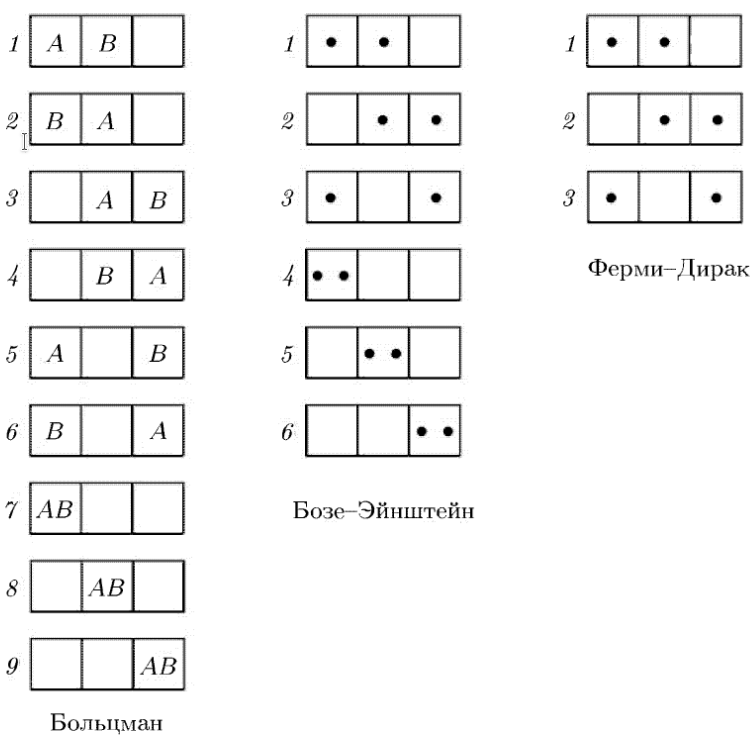
\includegraphics[width=0.85\linewidth]{stat_samples}}
		\caption{
			Примеры распределений.
		}
		\label{pic1}
	\end{figure}
	
	\tab На рис. \ref{pic1} видно, что между тремя статистиками имеются различия.
	
	\tab Решим задачу о распределении $N$ тождественных частиц по $Z$ квантовых состояний. Для \textit{фермионов} пусть будет $N$ занятых и $Z - N$ незанятых состояний ($Z \geq N$, иначе нерешаемо). Произведем всевозможные перестановки между ними, учитывая, что перестановки между занятыми и между незанятыми состояниями не приводят к новому макросостоянию. В итоге число перестановок, удовлетворяющих заданным условиям, будет равно $\cfrac{Z!}{N! (Z - N)!}$
	
	\tab Для \textit{бозонов} у нас имеется $Z$ <<клеток>>, $Z - 1$ <<перегородок>>, $N$ частиц. Всего $N + Z - 1$ элементов. Произведем перестановки между ними, учитывая, что перестановки между <<перегородками>> и между частицами не приводит к новому макросостоянию. В итоге число перестановок, соответствующих заданным условиям, будет равно $\cfrac{(Z + N - 1)!}{N! (Z - 1)!}$.
	Разделим все квантовые состояния на энергетические слои. Каждый слой состоит из квантовых состояний с близкими значениями энергии частиц. Для $i$-ого слоя:
	\begin{center}
		$G_i = \cfrac{Z_i!}{N_i! (Z_i - N_i)!}$ \tab\tab $G_i = \cfrac{(Z_i + N_i - 1)!}{N_i! (Z_i - 1)!}$
	\end{center}
	
	\tab Перемножая все $G_i$, найдем статистический вес макросостояния: $G = \prod\limits_i G_i$.
	
	\tab Найдем наиболее вероятные распределения. При больших $N_i$ и $Z_i$:
	$$
	S_{\text{ФД}} = -k \sum\limits_i\left[\ N_i \ln N_i + (Z_i - N_i) \ln (Z_i - N_i) \right] + C
	$$
	$$
	S_{\text{БЭ}} = -k \sum\limits_i \left[ (Z_i + N_i - 1) \ln (Z_i + N_i - 1) - N_i \ln N_i \right] + C
	$$
	
	\tab Из условия максимума энтропии и $\sum\limits_i N_i = N = \const,~ \sum\limits_i \mathcal{E}_i N_i = E = \const$:
	\begin{center}
		\begin{tabular}{l}
	$\mathlarger{\sum}\limits_i \ln \cfrac{N_i}{Z_i - N_i} ~ dN_i = 0$ \tab\tab (для фермионов) \\
	$\mathlarger{\sum}\limits_i \ln \cfrac{N_i}{Z_i + N_i - 1} ~ dN_i = 0$ \tab\tab (для бозонов) \vspace{0.2cm} \\
	$\sum\limits_i dN_i = 0$ \tab \tab $\sum\limits_i \mathcal{E}_i dN_i = 0$
		\end{tabular}
	\end{center}
	
	\tab $\Rightarrow \mathlarger\sum\limits_i \left( \ln \cfrac{N_i}{Z_i - N_i} + \beta + \alpha \mathcal{E}_i \right) dN_i = 0$ \tab (для фермионов).
	
	\tab \hphantom{$\Rightarrow$} $\mathlarger\sum\limits_i \left( \ln \cfrac{N_i}{Z_i + N_i - 1} + \beta + \alpha \mathcal{E}_i \right) dN_i = 0$ \tab (для бозонов).
	
	\tab Множители при $dN_i$ должны обратиться в нуль:
	\begin{center}
		\begin{tabular}{l}
			$\cfrac{\overline{N_i}}{Z_i - \overline{N_i}} = A e^{-\alpha \mathcal{E}_i}$ \tab (для фермионов). \\
			$\cfrac{\overline{N_i}}{Z_i + \overline{N_i}} = A e^{-\alpha \mathcal{E}_i}$ \tab (дя бозонов, $Z_i, N_i \gg 1$) \vspace{0.2cm} \\
			$\overline{n_i} = \cfrac{\overline{N_i}}{Z_i}~,$ \tab \tab $\alpha = \cfrac{1}{kT}$ \vspace{0.5cm} \\
			\fbox{$\overline{n_i} = \dfrac{1}{\exp\left({\dfrac{\mathcal{E}_i - \mu}{kT}}\right) + 1}$ \tab (для фермионов)} \vspace{0.2cm} \\
			\fbox{
			$\overline{n_i} = \dfrac{1}{\exp\left({\dfrac{\mathcal{E}_i - \mu}{kT}}\right) - 1}$ \tab (для бозонов) }
		\end{tabular}
	\end{center}
	
	\tab Здесь $\mu$ связано с $A$ соотношением: $A = \exp\left({\dfrac{\mu}{kT}}\right)$. Это и есть распределение Ферми-Дирака и Бозе-Эйнштейна. При $\overline{n_i} \ll 1$ оно переходит в распределение Больцмана:
	
	\tab $n_i \approx \exp\left(\dfrac{\mu - \mathcal{E}_i}{kT}\right) = C \exp\left( \dfrac{-\mathcal{E}_i}{kT} \right)$
	
	\tab Выведем свободную энергию $\Psi$ при постоянных $T, V$ в зависимости от $N$. При изменении $N$ $\mathcal{E}_i$ и $Z_i$ не меняются только числа заполнения $N_i$. Поэтому для приращения энтропии $S_\text{Ф}$: 
	
	\tab $d S_\text{Ф} = - K \sum\limits_i \ln \dfrac{N_i}{Z_i - N_i} dN_i$
	
	\tab В состоянии равновесия: $\ln \dfrac{N_i}{Z_i - N_i} = \dfrac{\mu - \mathcal{E}_i}{kT} \Rightarrow dS_\text{Ф} = - K \sum\limits_i \dfrac{\mu - \mathcal{E}_i}{kT}\, d\overline{N_i}$.\tab При этом $\sum\limits_i \mathcal{E}_i d\overline{N_i} = dU,~~ \sum\limits_i dN_i = dN$. Тогда $TdS_\text{Ф} = - \mu dN + dU, ~~ d\psi = \mu d N, ~~ \mu = \left( \dfrac{\partial \psi}{\partial N} \right)_{T,V}$, т.е. $\mu$ -- химический потенциал. Он определяется из условий нормировки:
	$$
	\sum\limits_i Z_i \overline{n_i} = \mathlarger\sum\limits_i \frac{Z_i}{\exp\left( \dfrac{\mathcal{E}_i - \mu}{kT} \right) \pm 1}
	$$
	но с точностью до произвольной постоянной, как и $\mathcal{E}_i$. Если энергию самого нижнего уровня принять за 0, то $\mu$ определится однозначно.
	
	\tab $\overline{n_i} \geq 0 \Rightarrow \mu \ll \mathcal{E}_i$ для бозе-газа, $\forall i$.
	
	\tab $i = 1, \mu \leq 0 $ (для Больцмана $\mu < 0$ из $n_i \ll 1$).
	
	\tab При $\mu > 0$ и $T \rightarrow 0$ для Ферми-Дирака имеем:
	$$
	\overline{n_i} \rightarrow \left\{
		\begin{array}{l}\
			1, ~\mathcal{E}_i < \mu \\
			\,\dfrac{1}{2}, ~\mathcal{E}_i = \mu \\
			\,0, ~\mathcal{E}_i > \mu
		\end{array}
		 \right.
	$$
	
	\tab При $T = 0$ частицы заполняют все состояния с энергией $\mathcal{E}_i < \mu$, состояния с более высокими энергиями не заняты - это называется состоянием полного вырождения.
	
		\begin{figure}[h]
			{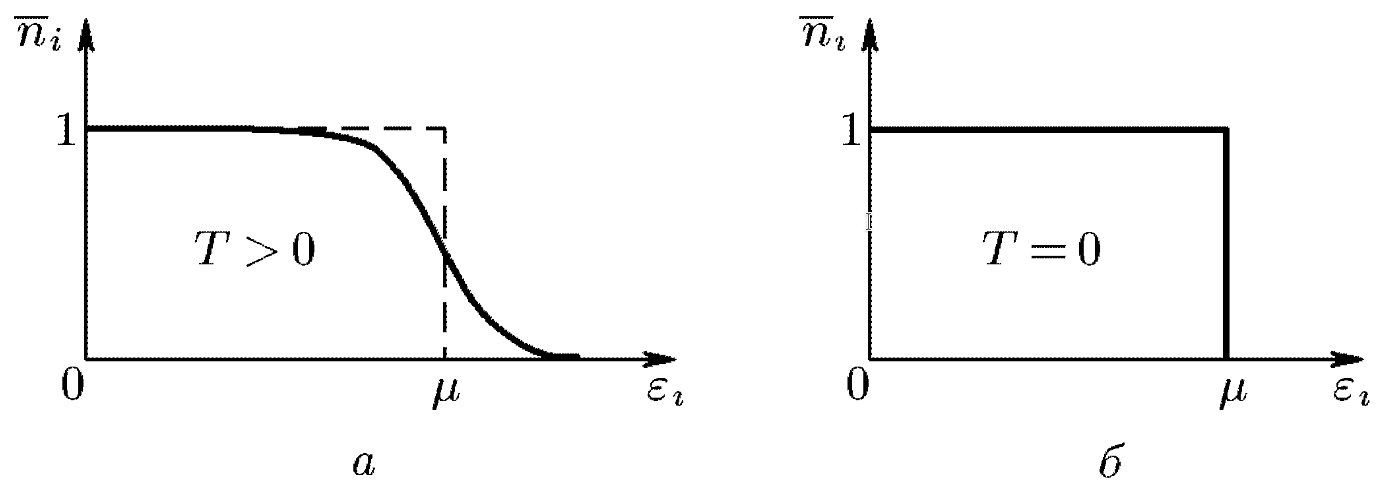
\includegraphics[width=0.85\linewidth]{graph1}}
			\caption{
				Зависимость $\overline{n_i}$ от $\mathcal{E}_i$ при $\mu > 0$.
			}
			\label{pic2}
		\end{figure}
		
			\begin{figure}[h]
				\center{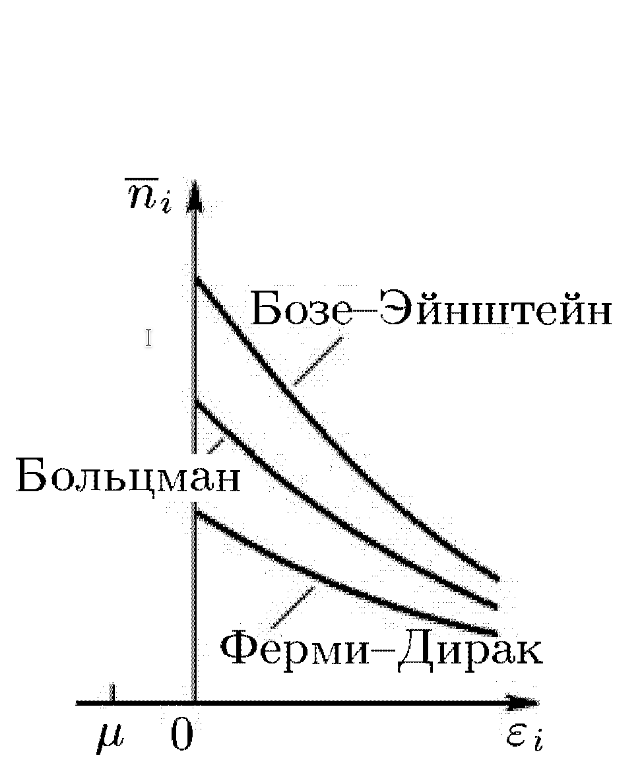
\includegraphics[width=0.3\linewidth]{graph2}}
				\caption{
					Сравнения распределений.
				}
				\label{pic3}
			\end{figure}
	
	\newpage \tab При $T \rightarrow 0$ для Бозе-Эйнштейна наблюдается явление Бозе-Эйнштейновской конденсации. При $T = 0 ~ \mu = 0$, все частицы накапливаются на нижнем квантовом уровне $\mathcal{E}_i = 0$
	
	\section{Применение}
	\tab Равновесное излучение как фотонный газ:
	$$
	\overline{n}(\mathcal{E}) = \dfrac{1}{\exp\left( \dfrac{\mathcal{E} - \mu}{kT} \right) - 1}
	$$
	
	\tab Число частиц переменно (фотоны могут излучаться и поглощаться в любом количестве).
	
	\tab Свободная энергия -- функция от $N, T, V$. Если при некоторых $T, V$ в газе содержится $N$ фотонов, то из условия минимума свободной энергии при равновесии:
	
	\tab $\left( \dfrac{\partial F}{\partial N} \right)_{V, T} = 0 \Rightarrow$ хим. потенциал $\mu = 0$
	
	\tab $\Rightarrow \overline{n}(\mathcal{E}) = \dfrac{1}{\exp\left( \dfrac{\mathcal{E}}{kT} \right) - 1} = \dfrac{1}{\exp\left( \dfrac{h\nu}{kT} \right) - 1}$~~. Это распределние Планка.
	
	\tab $g(\nu) d \nu = V \cdot \dfrac{4 \pi \nu^2 d\nu}{c^3}$ - стат. вес состояний в интервале частот от $\nu$ до $\nu + d\nu$.
	
	$$dN(\nu) = g(\nu)n(\nu) d\nu = \dfrac{V \cdot 8 \pi \nu^2 d\nu}{c^3 \left(\exp\left( \dfrac{h\nu}{kT} \right)\right) - 1}$$
	
	$$U = \int\limits_0^\infty dE(\nu) = V \cdot \sigma T^4,~~ \text{где } \sigma = \dfrac{8 \pi^5 k^4}{15 c^3 h^3}$$
	
	$$\dfrac{U}{V} = \sigma T^4 - \text{закон Стефана-Больцмана} $$
	
\end{document}